\documentclass[11pt]{article}
\usepackage{fullpage}
\usepackage[margin=2.5cm, bottom=3cm]{geometry}
\usepackage{amsmath,amsthm,amsfonts,amssymb,amscd}
\usepackage{mathrsfs}
\usepackage{fancyhdr}
\usepackage{multicol}
\usepackage{hyperref}
\usepackage{graphicx}
\usepackage[backend=biber]{biblatex}
\graphicspath{ {./../imgs/} }

\addbibresource{baby_cry.bib}

\hypersetup{
colorlinks=true,
linkcolor=blue,
linkbordercolor={0 0 1},
citecolor=black
}

\linespread{1.25}
\pagestyle{fancyplain}
\headsep 1.5em
\headheight 14pt

\title{Image Segmentation Using Markov Random Fields: An Implementation}

\author{Jake Callahan, James Griffin, McKay Harward, Taylor Paskett, Isaac Robbins, Mingyan Zhao}

\begin{document}

\begin{abstract}
The goal of this project was to evaluate current use of Markov random fields in image segmentation, then to implement one of the more advanced methods. In this paper we discuss how we implemented the equations from a paper based on an unsupervised method that used metropolis Hastings algorithm to find the best parameters for the Markov random field as well as the best number of classes. In short, we coded up a hands-off method of segmenting an input image.
\end{abstract}

\section{Background and Motivation}
This paper was motivated by the desire for a hands-off unsupervised image segmentation algorithm.
Our primary motivation for wanting a hands-off image segmenter had to do with applications in neural photo editing using introspective adversarial networks as well as image recognition.
The idea for using Markov random fields (MRF) for image segmentation is not new, in fact, the paper we decided to implement was written in 2000, but the unsupervised method doesn’t seem to have any study since then.
The background research we conducted only returned methods for segmenting images based on pretraining an MRF on a class, and then estimating which pixels in a given image are most likely to be of that class.
This included training the model to recognize trees and foilage, or roads using labeled images and then segmenting a new image based on the previous learned classes.
While this is useful, the hands-off approach can work in far more applications because it does not require labeled data.
The drawback of an unsupervised method is that it trades an initial investment of creating a pretrained MRF for a computationally expensive algorithm using Metropolis Hastings to update the MRF parameters.

We investigated numerous methods for performing unsupervised image segmentation, however, ran into many road blocks with many different papers.
The difficulty of these methods truly shocked us as we were unable to make any progress with numerous different papers.
This paper, although older and full of poor notation, at least provided a simple overview of the algorithm along with the equations necessary to implement it.
Anothe benefit of using the method described in this paper is that this paper does not require the user to specify the number of classes or segments.
Rather, the final step of this iterative algorithm samples the best number of classes using Bayesian statistics.


\section{Data}
The image segmentation algorithm that we implemented in this paper is an unsupervised method.
This means that the only data involved is the image that is segmented.
We use a few different images, the first being a simple noisy grid of 16 different colored squares used in the paper.
This served as a bit of a baseline to compare our results to those achieved in the paper.
We used a second simple image with only a few clear segments.
This image was used largely for testing the model as it was small and allowed us to run the model quickly.
Finally we used a few photographs to see the final results of our model.

\begin{figure}[!htb]
\begin{center}
\begin{multicols}{3}
    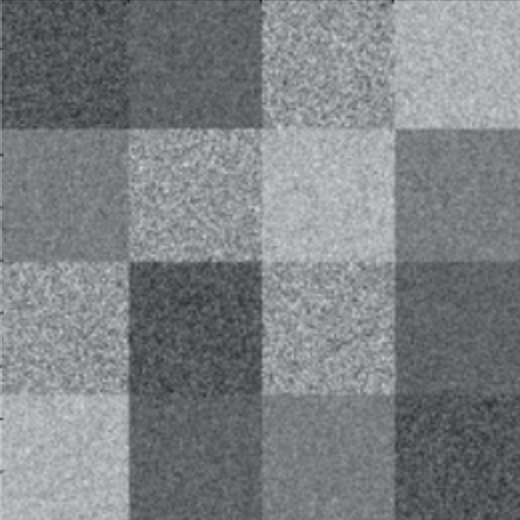
\includegraphics[height = \linewidth]{squares}\par
	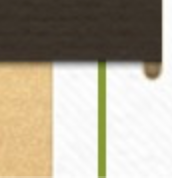
\includegraphics[height = \linewidth]{test}\
	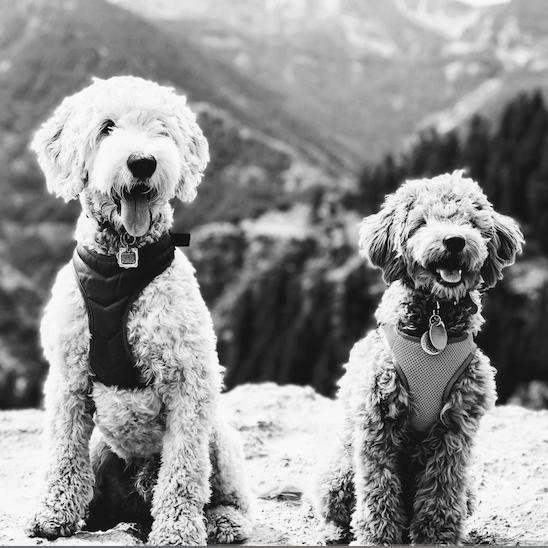
\includegraphics[height = \linewidth]{targetpractice}\par
\end{multicols}
\caption{The images used for training}
\end{center}
\end{figure}

\section{Methods}
Below is a simple overview of the algorithm proposed and then the modified algorithm we implemented.
A more in depth explanations of each step along with descriptions of how we implemented them and the difficulties we encountered at each step follows the algorithms.

\begin{enumerate}
	\item Randomly initialize the parameters for the MRF and number of classes
	\item Get the most likely segmentation given the MRF parameters
	\item Sample updated noise parameters $\mu$ and $\sigma$ for each class using Metropolis Hastings
	\item Sample updated MRF parameters $\beta_0$ and $\beta_1$ for each class using Metropolis Hastings
	\item Sample number of classes
	\item Repeat steps (2) - (5)
\end{enumerate}

Thought the process is simple, each of these steps required extensive coding and interpretation of the equations described in the paper.
Many of the equations were especially vague and incldued very poor and inconsistent notation which further complicated the already difficult equations.
Sampling the number of classes was the most complex section of the paper and the notation was especially difficult to understand.
We were unable to implement this step, however, this was not a major issue, because this only affected how many classes were being used and was a parameter we could fix.
Leaving this out, we ended up implementing the following method.

\begin{enumerate}
	\item Set the number of desired classes and randomly initialize the parameters for the MRF
	\item Get the most likely segmentation given the MRF parameters
	\item Sample updated noise parameters $\mu$ and $\sigma$ for each class using Metropolis Hastings
	\item Sample updated MRF parameters $\beta_0$ and $\beta_1$ for each class using Metropolis Hastings
	\item Repeat steps (2) - (4)
\end{enumerate}


Here is a overview of the variables used in the equations:

\begin{itemize}
	\item $\Omega$: The image being classified
	\item $s$: A pixel of the image $\Omega$
	\item $Y$: The grayscale image intensities
	\item $y_{s}$: The grayscale intensity at pixel $s$ in the interval $(0,1]$
	\item $X$: The segmentation labels for the MRF
	\item $x_{s}$: The class to which pixel $s$ is assigned
	\item $\Lambda$: The set of class labels
	\item $\eta_{s}$: The set of 4 direct neighbors of cell $s$
	\item $\Psi$: The parameter vector consisting of both noise and MRF parameters
	\item $\Theta_{c}$: The noise model parameter vector consisting of $\mu_{c}$ and $\sigma_{c}$
	\item $\beta_{c}^{(0)}$: The external field parameter
	\item $\beta_{c}^{(1)}$: The inter-pixel interaction strength parameter
	\item $T_{t}$: The annealing temperature at iteration $t$
	\item $n_{c}$: The number of pixels of class $c$
	\item $n_{(c, \eta)}$: Abusive notation explained in Section 3.3
\end{itemize}



\subsection{Segment the Image with the MRF}
\begin{equation}
\begin{aligned}
p\left(x_{s} = c | y_{s}, \eta_{s}, \Psi_{c}\right) & \propto \\
&\frac{1}{\sqrt{2 \pi \sigma_{c}^{2} T_{t}}} \exp \left\{ -\frac{1}{T_{t}} \left[\frac{1}{2} \left(\frac{y_{s}-\mu_{c}}{\sigma_{c}}\right)^{2} + \left( \beta_{c}^{(0)} + \beta^{(1)} V(c, \eta_{s}) \right) \right] \right\}
\end{aligned}
\end{equation}

where $V(c, \eta)=\frac{1}{4} \sum_{t \in \eta}(c \oplus\left.x_{t}\right),$ where $\oplus$ is an operator defined to take the value -1 if its arguments are equal, otherwise, +1.

With an initial set of random parameters to define our MRF, we needed to first find the probability of each pixel being in each class.
This was relatively simple to compute once the equation had been coded.
We then calculated the probabilities over the entire image for each class and took the argmax, thereby assigning each pixel to the class to which it most likely belongs.


\subsection{Update Noise Parameters}
The noise parameters $\mu_{c}$ and $\sigma_{c}$ are sampled using Metropolis-Hastings with the following likelihood:
\begin{equation}
\begin{aligned}
p\left(\mu_{c}, \sigma_{c} | Y, X\right) & \propto \prod_{s: x_{s}=c} p\left(y_{s} | \mu_{c}, \sigma_{c}\right) p_{r}\left(\mu_{c}\right) p_{r}\left(\sigma_{c}\right) \\
&=\frac{1}{\sigma_{c}\left(2 \pi \sigma_{c}^{2} T_{t}\right)^{n_{c}}} \exp \left\{-\frac{1}{2 T_{t}} \sum_{s: a_{s=c}}\left(\frac{y_{s}-\mu_{c}}{\sigma_{c}}\right)^{2}\right\}
\end{aligned}
\end{equation}

With a firm grasp on Metropolis Hastings, we expected updating the noise parameters to be straightforward, however, the suggested $T_{t}$ from the paper was so large, we ran into immediate underflow errors during computation.
We soon realized the issue was the $n_{c}$ exponent in the denominator causing our underflow.
While segmenting a small 100 x 100 image into 4 classes, $n_{c}$ should be about 25,000 and possibly much larger.
This necessitated that we calculate the equation in a completely different form which we give below.

\begin{equation}
\begin{aligned}
p\left(\mu_{c}, \sigma_{c} | Y, X\right) & \propto \frac{1}{\sigma_{c}}\prod_{s: x_{s}=c} \frac{1}{2 \pi \sigma_{c}^{2} T_{t}} \exp \left\{-\frac{1}{2 T_{t}} \left(\frac{y_{s}-\mu_{c}}{\sigma_{c}}\right)^{2} \right\}
\end{aligned}
\end{equation}

This allowed us to avoid the exponent and the large sum, both of which could cause massive underflow by calculating a each part of the product individually.
Because this probability would be used only for the acceptance ratio $a$ in the Metropolis Hastings algorithm, we extended this calculation one step further.

\begin{equation}
\begin{aligned}
a & = \frac{p\left(\mu_{c}^{new}, \sigma_{c}^{new} | Y, X\right)}{p\left(\mu_{c}, \sigma_{c} | Y, X\right)}\\ & \propto \prod_{s: x_{s}=c}  \frac{\frac{1}{2 \pi \sigma_{c}^{new2} T_{t}} \exp \left\{-\frac{1}{2 T_{t}} \left(\frac{y_{s}-\mu_{c}^{new}}{\sigma_{c}^{new}}\right)^{2} \right\}}{\frac{1}{2 \pi \sigma_{c}^{2} T_{t}} \exp \left\{-\frac{1}{2 T_{t}} \left(\frac{y_{s}-\mu_{c}}{\sigma_{c}}\right)^{2} \right\}}
\end{aligned}
\end{equation}

This allowed us to calculate the acceptance ratio for a single pixel before taking the product over all of the pixels of the specified class.
By doing so, we completely avoided underflow, however, we were only getting acceptance ratios of $0$ and $\infty$.
At first this concerned us but we realized that given model parameters, the these individual ratios would be very similar, at least across each class, thus for $a_{s} > 1$ taking the product would approach $\infty$ and for $a_{s} < 1$, the product would approach 0.
Having resolved this issue, we were able to update our noise parameters $\mu_{c}$ and $\sigma_{c}$ properly.

\subsection{Update MRF Parameters}
The MRF parameters $\beta_{c}^{(0)}$ are sampled using Metropolis-Hastings just like the previous step with the following probability:

\begin{equation}
\begin{array}{l}
p\left(\beta_{c}^{(0)}, c \in \Lambda | X\right) \\
\quad=p\left(X | \beta_{c}^{(0)}, c \in \Lambda\right) p_{r}\left(\beta_{c}^{(0)}, c \in \Lambda\right) \\
\quad=\prod_{\left(c \in \Lambda, \psi_{\eta}\right)}\left(\frac{\exp \left(-\frac{1}{T_{t}}\left[\beta_{c}^{(0)}+\beta^{(1)} V(c, \eta)\right]\right)}{\sum_{i \in \Lambda} \exp \left(-\frac{1}{T_{t}}\left[\beta_{i}^{(0)}+\beta^{(1)} V(i, \eta)\right]\right)}\right)^{n_{(c, \eta)}} \\
\quad=\prod_{(c \in \Lambda)}\left(\frac{\exp \left(-\frac{1}{T_{t}}\left[\beta_{c}^{(0)}\right]\right)}{\sum_{i \in \Lambda} \exp \left(-\frac{1}{T_{t}}\left[\beta_{i}^{(0)}\right]\right)}\right)^{n_{c}} \\
\quad \times \prod_{(c \in \Lambda, \psi \eta)}\left(\frac{\exp \left(-\frac{1}{T_{t}}\left[\beta^{(1)} V(c, \eta)\right]\right) \sum_{i \in \Lambda} \exp \left(-\frac{1}{T_{t}}\left[\beta_{i}^{(0)}\right]\right)}{\sum_{i \in \Lambda} \exp \left(-\frac{1}{T_{t}}\left[\beta_{i}^{(0)}+\beta^{(1)} V(i, \eta)\right]\right.}\right)^{n_{(c, \eta)}}
\end{array}
\end{equation}

We immediately ran into the issue of the definition of the exponent $n_{(c, \eta)}$ that is used.
The paper defines this as $n_{(c, \eta)}=\#\left(s: x_{s}=c, \eta_{s}=\eta\right)$
This notation is abusive and does not follow what had been previously done.
After much deliberation, we realized that this was an extremely convoluted way of iterating over each $s:x_{s} = c$ as they had done in all previous equations.
For no apparent reason they were iterating over $\eta$ with a counting function that returned $n_{(c, \eta)}=0$ if $x_{s} \neq c$ and $n_{(c, \eta)}=1$ if $x_{s} = c$. Thus the probabilities corresponding to pixels such that $x_{s} \neq c$ were set to $1$ and essentially excluded from the product.
We remedied this equation as follows:

\begin{equation}
\begin{aligned}
p\left(\beta_{c}^{(0)}, c \in \Lambda | X\right) & = \prod_{s:x_{s} = c}\frac{\exp \left(-\frac{1}{T_{t}}\left[\beta_{c}^{(0)}+\beta^{(1)} V(c, \eta_{s})\right]\right)}{\sum_{i \in \Lambda} \exp \left(-\frac{1}{T_{t}}\left[\beta_{i}^{(0)}+\beta^{(1)} V(i, \eta_{s})\right]\right)}
\end{aligned}
\end{equation}

This greatly simplified the calculations for updating the MRF parameters  $\beta_{c}^{(0)}$.
We used the same method as described in Section 3.2 of calculating each of the individual acceptance ratios $a_{s}$ before taking the product over all the ratios.
A similar equation is proposed for the likelihod $p(\beta_{c}^{(1)}, c \in \Lambda | X)$, however, the paper states that the posterior density alculation for $\beta_{c}^{(1)}$ will not be proper under particular underlying label map configurations.
The paper fixes a value \textit{a priori} of $1.5$ for $\beta_{c}^{(1)}$.
We follow this practice in our approach.

\subsection{Number of classes}
The most difficult part of this paper involved sampling the number of classes.
The notation throughout this part of the paper was very difficult to understand.
Below is the equation for the acceptance ratio for splitting a class $c$ into $c_{1}$ and $c_{2}$.

\begin{equation}
\begin{aligned}
\frac{p\left(X=x^{+}, \psi^{+}, k^{+} | Y=y\right)}{p(X=x, \psi, k | Y=y)} & \frac{1}{p_{\beta}\left(u_{1}\right) p_{\beta}\left(u_{2}\right) p_{\beta}\left(u_{3}\right)} \\
\times \frac{\partial\left(\Psi_{c 1}, \Psi_{c 2}\right)}{p(\text {segmentation})} &\left|\frac{1}{\partial\left(\Psi_{c}, u_{1}, u_{2}, u_{3}\right)}\right|
\end{aligned}
\end{equation}

Unfortunately, we were never able to work out the notation in a way that made enough sense to even try and implement this sampling.
However, this step only helps find the optimal number of classes for the segmentation at each step and emmitting this step should not affect the other steps or performance of the algorithm as a whole.
With this step omitted from the algorithm, we simply specify the desired number of classes before running it.

\section{Results}


\section{Analysis}
Our methods turned out to be fairly effective. They don’t par with current state of the art technologies but they definitely do well for something done by a few undergraduate students in a single project, not research. The model we’ve created does a fairly decent job of segmenting images on par with what the original authors achieved, though sometimes in a few extra iterations. Looking at how it works, I do think it would work in a GAN for neural photo editing to maybe train the GAN to focus itself more closely on one area while keeping the rest of the image the same, but even with faster computers, it seems it still takes too long for any practical applications. Given enough computing power it can be used.

\section{Conclusion}
The initial intent of getting a completely unsupervised method of image segmentation using Markov Random Fields was successful and could probably be improved upon for efficiency. If given the opportunity to try image segmentation again, I would probably opt to use a neural network as they tend to require an initial investment of training time but can then be used to segment an image very quickly. Something we could do is have more informed priors for each parameters. We could also implement for color images (may be?)


\end{document}
